\makeatletter
\def\input@path{{./Graphics/}} % Définition du chemin d'entrée pour les graphiques
\makeatother

\documentclass[12pt,a4paper]{article} % Classe de document

% Chargement des packages essentiels
\usepackage[utf8]{inputenc} % Encodage UTF-8
\usepackage[french]{babel} % Support de la langue française
\usepackage{graphicx, amsthm, mathtools, amsfonts, amssymb, physics, longtable, mathrsfs} % Packages pour les graphiques et mathématiques

\usepackage{float} % Gère le placement des objets flottants
\floatplacement{figure}{H} % Forces les figures à être placées exactement à l'endroit où elles apparaissent dans le texte

\usepackage[svgnames,x11names,rgb,table]{xcolor} % Définit les couleurs par noms
\usepackage{array, multicol, wrapfig, lmodern, multirow, booktabs, chemformula} % Diverses améliorations de mise en forme
\usepackage[detect-all=true, group-minimum-digits=4]{siunitx} % Pour les unités SI

\usepackage[bf, textfont={footnotesize,it}]{caption} % Personnalisation des légendes
\usepackage{subcaption}

% Configuration des marges de la page
\usepackage[margin=2cm, a4paper]{geometry}

\usepackage{fancyvrb} % Remplacement du mode verbatim qui permet une meilleure mise en forme
%\usepackage[Export]{adjustbox} % Utilisé pour contraindre les images à une taille maximale
%\adjustboxset{max size={0.9\linewidth}{0.9\paperheight}} % Taille maximale des images

% Configuration pour hyperref
\usepackage{hyperref} 
\hypersetup{
    colorlinks=true, % Colorise les liens
    breaklinks=true, % Permet le retour à la ligne dans les liens trop longs
    allcolors=Blue3, % Couleur des liens
    pdfauthor={Nana Engo}, % Auteur du document PDF
    pdfsubject={Chimie quantique et VQE}, % Sujet du document
    pdftitle={PHY4268 - Chimie quantique et VQE V25.03}, % Titre du document
    bookmarksopen=true % Ouvre les signets PDF par défaut
}

\usepackage{cleveref} % Améliore la gestion des références croisées

\frenchbsetup{StandardLayout=true} % Configuration du layout français
\numberwithin{equation}{section} % Numérotation des équations par section
\numberwithin{figure}{section} % Numérotation des figures par section
\numberwithin{table}{section} % Numérotation des tables par section

\setcounter{secnumdepth}{3} % Pour inclure les sous-sections
\renewcommand{\thesection}{\arabic{section}} % Numérotation des sections
%
\newcommand{\tcb}[1]{\textcolor{blue}{#1}} % textcolor{blue}{#1}
\newcommand{\tcr}[1]{\textcolor{red}{#1}} % textcolor{red}{#1}
% Titre du document
\title{\vspace*{4cm}
\Huge\tcb{Chapter 1 - Quantum Chemistry Modelling Basis}
\vspace*{5cm}}

\author{
\begin{tabular}{lr}
    \textbf{Nana Engo} & \textbf{Tchapet Njafa}\\
    {\small  serge.nana-engo@facsciences-uy1.cm} &\hspace*{2em}
    {\small jean-pierre.tchapet@facsciences-uy1.cm}
\end{tabular}\\[3em] % Espace entre les auteurs et la filiation
\textit{Quantum Simulation Group}\\
    \textit{Department of Physics} \\ 
    \textit{Faculty of Science} \\ 
    \textit{University of Yaoundé I}
}
\date{\vspace*{3cm}March 2025} % Date du document

\begin{document}
\maketitle % Affiche le titre, les auteurs et la date

\newpage
\section{Introduction}

La chimie quantique est une discipline fondamentale qui permet de décrire et de prédire les propriétés électroniques et structurales des systèmes atomiques et moléculaires à l'aide des principes de la physique quantique. Elle constitue un outil essentiel pour comprendre les interactions chimiques, modéliser les réactions complexes et développer des applications pratiques dans des domaines variés tels que la conception de nouveaux matériaux, l'optimisation des processus chimiques ou encore le développement de médicaments.

Avec l'émergence des technologies computationnelles modernes et des algorithmes avancés comme le \emph{Variationnel Quantum Eigensolver} (VQE), la chimie quantique computationnelle a révolutionné la recherche scientifique et industrielle. Ces approches permettent de simuler efficacement des systèmes complexes en exploitant des approximations telles que l'approximation de Born-Oppenheimer (BO) ou la méthode Hartree-Fock (HF), tout en maintenant un équilibre entre précision et faisabilité computationnelle.

Dans ce chapitre, nous introduisons les concepts fondamentaux suivants :
\begin{itemize}
    \item L'Hamiltonien moléculaire en première quantification ;
    \item L'approximation de Born-Oppenheimer ;
    \item L'approche du champ moyen via la méthode Hartree-Fock (HF) ;
    \item Les limites inhérentes à cette méthode ;
    \item Le choix et l'importance des ensembles de bases.
\end{itemize}

Ces notions sont illustrées par leur rôle dans le workflow de l'algorithme VQE (voir les encadrées en rouge sur la \autoref{fig:VQE_Flowchart}), qui constitue une avancée majeure pour les simulations moléculaires en chimie quantique. Ces méthodes ont de nombreuses applications pratiques, notamment dans le domaine énergétique (\autoref{fig:CoverVQE}) , où elles contribuent au développement de matériaux innovants et à l'optimisation des processus chimiques.

Ce chapitre vise à fournir une base solide pour comprendre les principes sous-jacents à la modélisation chimique en physique quantique, tout en mettant en lumière les défis computationnels et les opportunités offertes par ces approches modernes.

\begin{figure}
\centering

\includegraphics[width=.9\linewidth]{VQE_Flowchart.jpeg} 
\caption{\textbf{Diagramme de flux de l'algorithme VQE (Variationnel Quantum Eigensolver).} Ce diagramme illustre les étapes principales de l'algorithme VQE, une méthode hybride quantique-classique utilisée pour calculer l'énergie des molécules. On y voit comment une boucle itérative optimise les paramètres d'un circuit quantique (ansatz) afin de minimiser l'énergie, en utilisant un calculateur classique pour le contrôle et l'analyse des résultats quantiques. Les encadrés rouges mettent en évidence les contributions des concepts fondamentaux présentés dans ce chapitre, comme l'Hamiltonien moléculaire et l'approximation de Born-Oppenheimer.}
\label{fig:VQE_Flowchart}
\end{figure}

\begin{figure}
\centering

\includegraphics[width=.4\linewidth]{CoverVQE.jpg}
\caption{\textbf{Applications de la chimie quantique computationnelle dans le domaine de l'énergie.} Parmi celles-ci, on retrouve la conception de nouveaux matériaux pour les cellules solaires, l'optimisation des réactions catalytiques pour la production d'énergie propre, le développement de batteries plus performantes et la compréhension des mécanismes de stockage de l'énergie. Ces applications montrent le potentiel de la chimie quantique pour résoudre les défis énergétiques actuels.}
\label{fig:CoverVQE}
\end{figure}

\section{Hamiltonien moléculaire en première quantification}

\begin{figure}
\centering

\includegraphics[width=0.7\linewidth]{Interaction_QC.pdf}
\caption{\textbf{Illustration simplifiée des différentes interactions dans un système moléculaire.} Ce diagramme schématise les interactions fondamentales présentes dans une molécule, incluant les attractions et répulsions électrostatiques. On distingue les interactions entre les électrons et les noyaux (attraction), les répulsions entre les électrons et les répulsions entre les noyaux. Les étiquettes sur le schéma mettent en évidence la nature Coulombienne de ces interactions et montrent comment ces forces contribuent à l'énergie totale du système. La figure aide à visualiser les composantes de l'Hamiltonien moléculaire avant l'application de l'approximation de Born-Oppenheimer.}
\label{fig:interactionqc}
\end{figure}

La modélisation de la structure électronique des molécules est un problème complexe en raison du grand nombre de particules en interaction. La chimie quantique fournit un cadre théorique pour aborder ce problème, en utilisant l'équation de Schrödinger dépendante du temps suivante :
\begin{equation}
i\hbar \pdv{t} |\psi(t)\rangle = \mathtt{H} |\psi(t)\rangle .
\end{equation}
$|\psi(t)\rangle$ représente la fonction d'état du système, décrivant son évolution temporelle, et $\mathtt{H}$ est l'opérateur Hamiltonien, qui représente l'énergie totale du système. Résoudre cette équation directement, même en l'absence d'effets relativistes, reste un défi majeur pour les systèmes moléculaires complexes.

Pour simplifier, on se concentre souvent sur les états stationnaires du système. Ces états sont décrits par l'équation de Schrödinger \textit{indépendante} du temps, qui prend la forme d'un problème aux valeurs propres :
\begin{equation}
\mathtt{H} |\psi\rangle = E |\psi\rangle ,
\end{equation}
où $E$ représente l'énergie de l'état stationnaire $|\psi\rangle$. La résolution de cette équation nous permet de déterminer les énergies permises et les fonctions d'état associées à ces états.

L'Hamiltonien moléculaire, noté $\mathtt{H}$, décrit l'énergie totale d'une molécule constituée de $M$ noyaux et de $N$ électrons. Il englobe les énergies cinétiques et potentielles de toutes les particules en interaction. De manière générale, il peut être exprimé comme la somme des termes suivants (voir la \autoref{fig:interactionqc}):
\begin{equation}
\mathtt{H}=\mathtt{T}_e+\mathtt{T}_n+\mathtt{U}_{en}+\mathtt{U}_{en}+\mathtt{U}_{nn},
\end{equation}
où
\begin{itemize}
\item $\mathtt{T}_e= -\sum_i\frac{\hbar^2}{2m_e}\nabla^2_i$ est l'énergie cinétique électronique. Les électrons sont en mouvement constant autour des noyaux, ce qui contribue à l'énergie totale; 
\item $\mathtt{T}_n=-\sum_I\frac{\hbar^2}{2M_I}\nabla^2_I$ est l'énergie cinétique nucléaire. Les noyaux sont également en mouvement (vibrations, rotations), mais leur contribution est souvent négligeable en première approximation (Born-Oppenheimer); 
\item $\mathtt{U}_{en}= -\sum_{i,I}\frac{e^2}{4\pi\epsilon_0}\frac{Z_I}{|\mathbf{r}_i-\mathbf{R}_I|}$ est l'énergie potentielle d'attraction Coulombienne entre les électrons et les noyaux. C'est cette interaction \textbf{attractive Coulombienne} entre les électrons négatifs et les noyaux positifs qui stabilise la molécule;
\item $\mathtt{U}_{ee}=+\frac{1}{2}\sum_{i\neq j}\frac{e^2}{4\pi\epsilon_0}\frac{1}{|\mathbf{r}_i-\mathbf{r}_j|}$ est l'énergie potentielle de répulsion Coulombienne entre les électrons. Les électrons, portant la même charge négative, se repoussent mutuellement;
\item $\mathtt{U}_{nn}=+\frac{1}{2}\sum_{I\neq J}\frac{e^2}{4\pi\epsilon_0}\frac{Z_IZ_J}{|\mathbf{R}_I-\mathbf{R}_J|}$ est l'énergie potentielle de répulsion Coulombienne entre les noyaux.  Les noyaux positifs se repoussent. Cette répulsion est \textit{purement classique} et dépend uniquement de la distance internucléaire.
\end{itemize}
Dans ces expressions, $i$ et $j$ sont des indices qui parcourent tous les électrons, tandis que $I$ et $J$ parcourent tous les noyaux. Les variables $M_I$, $\mathbf{R}_I$, et $Z_I$ désignent respectivement la masse, la position et le numéro atomique du \emph{I}-ième noyau, tandis que $\mathbf{r}_i$ est la position du \emph{i}-ième électron.

Pour simplifier les calculs et faciliter l'interprétation des résultats, il est courant de travailler en unités atomiques. Dans ce système d'unités, l'unité de longueur est le Bohr ($a_0 \approx \SI{0.529167e-10}{\meter}$), l'unité de masse est la masse de l'électron ($m_e$), et l'unité d'énergie est le Hartree (\SI{1}{Hartree} $= \frac{e^2}{4\pi\epsilon_0 a_0} \approx \SI{27.2113}{\electronvolt}$). L'utilisation de ces unités simplifie les équations en fixant certaines constantes physiques à 1.

En définissant $M_I' = M_I / m_e$, les différents termes de l'Hamiltonien moléculaire s'expriment en unités atomiques comme suit :
\begin{equation}
\begin{split}
\mathtt{T}_e&=-\sum_i\frac{\nabla^2_i}{2}, \qquad\mathtt{T}_n= -\sum_I\frac{\nabla^2_I}{2M_I'}, 
 \qquad\mathtt{U}_{en}= - \sum_{i,I}\frac{Z_I}{|\mathbf{r}_i-\mathbf{R}_I|},\\
\mathtt{U}_{ee}&=+\frac12\sum_{i\neq j}\frac{1}{|\mathbf{r}_i-\mathbf{r}_j|}
=+\sum_{i,j>i}\frac{1}{|\mathbf{r}_i-\mathbf{r}_j|}=+\sum_{i,j>i}\frac{1}{r_{ij}},\\
\mathtt{U}_{nn}&=+\frac12\sum_{I\neq J}\frac{Z_IZ_J}{|\mathbf{R}_I-\mathbf{R}_J|}
=+\sum_{I,J>I}\frac{Z_IZ_J}{|\mathbf{R}_I-\mathbf{R}_J|}=+\sum_{I,J>I}\frac{Z_IZ_J}{R_{IJ}}.
\end{split}
\end{equation}

Cependant, la résolution directe de l'équation de Schrödinger avec cet Hamiltonien complet est extrêmement complexe, voire impossible, pour les systèmes moléculaires de taille significative. Cette complexité découle des interactions corrélées entre les nombreux électrons et noyaux. Pour surmonter cette difficulté, des approximations sont indispensables.

\section{Approximation de Born-Oppenheimer}\label{approximation-de-born-oppenheimer}

L'\textbf{approximation de Born-Oppenheimer} (BO) est une hypothèse fondamentale en chimie quantique, qui simplifie considérablement le traitement des systèmes moléculaires complexes. Elle repose sur la différence significative de masse entre les noyaux et les électrons. Les noyaux, étant bien plus massifs que les électrons ($M'\sim10^3$), se déplacent beaucoup plus lentement. Cette disparité dynamique permet de séparer les mouvements électroniques et nucléaires lors de la résolution de l'équation de Schrödinger (voir la \autoref{fig:bointeractionqc}). En d'autres termes, on considère que les électrons s'adaptent instantanément aux mouvements des noyaux, ce qui permet de découpler leurs équations de mouvement.

\begin{figure}
\centering

\includegraphics[width=0.7\linewidth]{BO_Interaction_QC.pdf}
\caption{\textbf{Illustration des interactions dans l'approximation de Born-Oppenheimer.} Ce schéma met en évidence la séparation des mouvements rapides des électrons et des mouvements lents des noyaux, due à la grande différence de masse entre ces particules. Les électrons sont considérés comme se déplaçant dans un champ créé par les noyaux fixes, ce qui permet de simplifier considérablement les calculs de structure électronique.
}
\label{fig:bointeractionqc}
\end{figure}

\subsection{Hamiltonien réduit}

En appliquant cette approximation,
\begin{itemize}
\item le terme d'énergie cinétique nucléaire $T_n$ est négligé; 
\item De plus, l'énergie de répulsion nucléaire $\mathtt{U}_{nn}(\mathbf{R})$ devient constante pour une géométrie nucléaire donnée.
\end{itemize}  
L'Hamiltonien électronique est alors extrait de l'Hamiltonien total:
\begin{equation}
\begin{split}
\mathtt{H}_{\text{elec}}(\mathbf{R}) &= \underset{\text{One-Electron Operators}}{\mathtt{T}_e + \mathtt{U}_{en}(\mathbf{R})} + \underset{\text{Two-Electron Operator}}{\mathtt{U}_{ee}}\\
&= \underset{\text{One-Electron Operator}}{\sum_i h(i)} + \underset{\text{Two-Electron Operator}}{\sum_{i\ne j}v(i, j)}\\
&=-\sum_{i=1}^N \frac12 \nabla_i^2 - \sum_{i=1}^N \sum_{A=1}^M \frac{Z_A}{r_{iA}} + \sum_{i=1}^N \sum_{j>i} \frac{1}{r_{ij}} .
\end{split}
\end{equation}
C'est cet Hamiltonien, agissant sur les électrons, que l'on cherche à résoudre pour une géométrie nucléaire fixée. Il faut bien comprendre que, sous BO, l'énergie des électrons dépend paramétriquement de la position des noyaux. Pour une configuration nucléaire donnée, on peut donc calculer l'énergie électronique $(E_{\text{elec}})$ en résolvant l'équation de Schrödinger électronique :
\begin{equation}
\mathtt{H}_{\text{elec}}(\mathbf{R}) \psi_{\text{elec}}(\mathbf{r}; \mathbf{R}) = E_{\text{elec}}(\mathbf{R}) \psi_{\text{elec}}(\mathbf{r}; \mathbf{R})
\end{equation}
où $\psi_{\text{elec}}(\mathbf{r}; \mathbf{R})$ est la fonction d'état électronique qui dépend des coordonnées électroniques ($\mathbf{r}$) et paramétriquement des coordonnées nucléaires ($\mathbf{R}$).

\subsection{Énergie totale du système}

La résolution de l'équation de Schrödinger électronique pour toutes les positions des noyaux permet de construire la \textbf{surface d'énergie potentielle (PES, 
Potential energy surface)}, $E_{\text{elec}}(\mathbf{R})$ (voir la \autoref{fig:PES}). Cette surface décrit l'énergie du système en fonction des positions des 
noyaux et est un concept central en chimie quantique.

\begin{figure}
\centering

\includegraphics[width=0.4\linewidth]{PES_H2.pdf}
\caption{\textbf{Surface d'énergie potentielle (PES).} Elle peut être utilisée pour explorer théoriquement les propriétés des structures composées d'atomes, par exemple pour trouver la forme d'énergie minimale d'une molécule ou pour calculer la vitesse d'une réaction chimique. Ici la courbe d'énergie potentielle est celle de la liaison covalente dans une molécule de $H_2$, générée dans le cadre d'un potentiel de Morse.
}
\label{fig:PES}
\end{figure}

Une fois l'énergie électronique obtenue, l'énergie totale est approchée comme suit :
\begin{equation}
E_{\text{tot}} = E_{\text{elec}} + E_{nn},
\end{equation}
où,
\begin{itemize}
\item $E_{\text{elec}}$ est l'énergie électronique, obtenue par la résolution de l'équation de Schrödinger électronique;
\item $E_{nn}=\sum_{A=1}^M \sum_{B>A} \frac{Z_A Z_B}{R_{AB}}$ représente l'énergie de répulsion entre les noyaux, considérés comme des charges ponctuelles fixes.
\end{itemize}

\subsection{Conséquences de l'approximation}

L'approximation de Born-Oppenheimer a des implications importantes :
\begin{itemize}
\item L'énergie totale est calculée pour une géométrie nucléaire fixe.  Cette simplification permet de déterminer les structures moléculaires à l'équilibre en minimisant l'énergie totale par rapport aux positions des noyaux.
\item Les mouvements des noyaux (vibration, rotation, translation) peuvent être traités séparément en utilisant un Hamiltonien nucléaire effectif :
\begin{equation}
\mathtt{H}_{\text{nucl}} = \mathtt{T}_n + E_{\text{tot}}(\{R_A\}) ,
\end{equation}
où $E_{\text{tot}}(\{R_A\})$ agit comme un potentiel pour le mouvement des noyaux. Ceci permet d'étudier les spectres vibrationnels des molécules.
\end{itemize}

En résumé, l'approximation de Born-Oppenheimer est essentielle pour séparer les degrés de liberté nucléaires et électroniques, rendant ainsi le problème beaucoup plus gérable en chimie quantique computationnelle. Bien qu'elle repose sur une simplification, elle fournit une base solide pour la compréhension et la prédiction des propriétés moléculaires. Il est cependant important de noter que cette approximation peut devenir moins précise dans certaines situations, notamment
\begin{itemize}
\item lorsque les surfaces d'énergie potentielle sont proches;
\item lorsqu'on étudie des processus dynamiques où le couplage entre les mouvements électroniques et nucléaires devient important.
\end{itemize}

\section{Méthode de Hartree-Fock - Approche du champ moyen}

La méthode de Hartree-Fock (HF) est une approche fondamentale qui approxime l'interaction électron-électron dans un système moléculaire en chimie quantique computationnelle. En réalité, résoudre directement l'équation de Schrödinger pour une molécule est impossible à cause des interactions complexes entre tous les électrons. L'astuce de Hartree-Fock est de remplacer ces interactions complexes par une approximation plus simple : le \textbf{champ moyen} ou \textbf{mean-field} en anglais.

Imaginez un électron qui se déplace dans une molécule. Au lieu de ressentir l'influence instantanée de tous les autres électrons, qui se déplacent aussi, on considère que cet électron se déplace dans un potentiel \textbf{moyen}, une sorte de \textbf{moyenne de l'influence de tous les autres électrons}.

En d'autres termes, au lieu de traiter le problème à N corps (N électrons), on le réduit à N problèmes à un seul corps, où chaque électron se déplace dans un potentiel effectif. Ce potentiel est dit \textbf{auto-cohérent} car il est déterminé par les orbitales des autres électrons.

Cette approximation a des conséquences importantes :
\begin{itemize}
    \item elle simplifie considérablement les calculs, rendant possible la modélisation de molécules plus grandes (\textbf{avantage principal});
    \item elle inclut les effets d'échange dus au principe de Pauli;
    \item elle néglige la \textbf{corrélation électronique dynamique}, c'est-à-dire la façon dont les électrons ajustent instantanément leur position les uns par rapport aux autres (\textbf{limite principale}).
\end{itemize}

Pour comprendre comment implémenter cette idée, il faut détailler comment on représente l'état quantique de la molécule.

\subsection{Fonction d'état - Déterminant de Slater}

L'approximation centrale de la méthode HF consiste à représenter la fonction d'état multi-électronique par un \textbf{déterminant de Slater}, qui encode mathématiquement l'antisymétrie requise pour les fermions que sont les électrons, particules de spin-$\frac12$. Il est défini comme suit :
\begin{equation}
\begin{split}
\psi(\mathbf{r}_0, \mathbf{r}_1, \ldots, \mathbf{r}_{N-1})\equiv |\phi_{M-1},\cdots,  \phi_1, \phi_0 \rangle 
&=   \frac{1}{\sqrt{N!}}
\begin{vmatrix} \phi_0(\mathbf{r}_0) & \phi_1(\mathbf{r}_0) & \cdots & \phi_{M-1}(\mathbf{r}_0) \\
      \phi_0(\mathbf{r}_1) & \phi_1(\mathbf{r}_1) & \cdots & \phi_{M-1}(\mathbf{r}_1) \\
      \vdots & \vdots & \ddots & \vdots \\
      \phi_0(\mathbf{r}_{N-1}) & \phi_1(\mathbf{r}_{N-1}) & \cdots & \phi_{M-1}(\mathbf{r}_{N-1})
\end{vmatrix} \\
&\equiv |M-1,\dots, 1, 0 \rangle,
\end{split}
\end{equation} 
Il est à noter que:
\begin{itemize}
\item $\mathbf{r}_i$ est la position de l'électron $i$;
\item $\phi_i$ est une \textbf{spin-orbitale}, c'est-à-dire une fonction décrivant à la fois la position spatiale et le spin d'un électron;
\item le déterminant assure que la fonction d'état est \textbf{antisymétrique} par rapport à l'échange de deux électrons (principe de Pauli). En d'autres termes, si on échange deux lignes dans le déterminant, la fonction d'état change de signe.
\end{itemize}

\textbf{Pourquoi un déterminant ?} Le déterminant de Slater est la \textit{façon la plus simple} de construire une fonction d'état multi-électronique qui respecte le principe fondamental de Pauli, qui stipule que la fonction d'état doit être antisymétrique par rapport à l'échange de deux fermions (les électrons sont des fermions).

Bien que le nombre de spin-orbitales considérées, $M$, soit généralement plus élevé que le nombre d'électrons dans le système, $N$, les électrons ne peuvent occuper que $N$ des spin-orbitales dans un déterminant de Slater donné. En conséquence, le déterminant de Slater ne contient que les spin-orbitales occupées $N$.


\subsubsection{Combinaison Linéaire d'Orbitales Atomiques (LCAO)}


Dans la base des \textbf{orbitales moléculaires (MO)}, chaque spin-orbitale $\phi_p(\mathbf{r})$ est une combinaison linéaire des \textbf{orbitales atomiques (AO)} via la méthode \textbf{LCAO} (Linear Combination of Atomic Orbitals):
\begin{equation}
\phi_p(\mathbf{r}) = \sum_\alpha c_{\alpha p} \chi_\alpha(\mathbf{r} - \mathbf{R}_\alpha),
\end{equation}
où $\mathbf{R}_\alpha$ représente la position du centre atomique de la fonction de base $\chi_\alpha$, et les coefficients d'expansion $c_{\alpha p}$ sont appelés \textbf{coefficients des orbitales moléculaires (OM)}. Ces coefficients $c_{\alpha p}$ déterminent la contribution de chaque orbitale atomique $\chi_\alpha$ à l'orbitale moléculaire $\phi_p$.

En utilisant la notation de Dirac, cette expansion LCAO prend la forme plus compacte :
\begin{equation}
  \ket{\phi_p} = \sum_\alpha c_{\alpha p}\ket{\chi_\alpha}.
\end{equation}

Il peut être pratique de regrouper l'ensemble des orbitales moléculaires (et atomiques) sous forme de vecteurs lignes.  Introduisons la notation suivante pour représenter un vecteur ligne d'orbitales moléculaires :
\begin{equation}
    \ket{\overline{\phi}} = (\ldots, \ket{\phi_p}, \ldots)
\end{equation}
L'expansion LCAO pour l'ensemble des orbitales moléculaires peut alors être écrite de manière encore plus concise sous forme matricielle :
\begin{equation}
    | \overline{\phi} \rangle = | \overline{\chi} \rangle \mathbf{C},
\end{equation}
où $\mathbf{C}$ est la \textbf{matrice des coefficients des orbitales moléculaires (OM)}. Chaque colonne de la matrice $\mathbf{C}$ contient les coefficients d'expansion LCAO pour une orbitale moléculaire donnée, et chaque ligne correspond à une orbitale atomique de base.

Cette expansion LCAO, bien qu'approximative, permet de transformer le problème de la résolution de l'équation de Schrödinger pour les électrons en un problème algébrique matriciel, qui peut être résolu numériquement sur ordinateur. Le choix des orbitales atomiques de base $\chi_\alpha$ (appelées aussi \textbf{ensembles de bases}) est un aspect essentiel de la modélisation moléculaire, que nous aborderons plus en détail dans la \autoref{sec:Base}.


\subsubsection{Spin et Déterminants de Slater}

Les déterminants de Slater, en plus d'assurer l'antisymétrie de la fonction d'onde, possèdent des propriétés importantes en ce qui concerne le spin électronique total du système.

\paragraph{Déterminants et Spin $S_z$}

Tous les déterminants de Slater sont des fonctions propres de l'opérateur $ \mathtt{S}_z$, qui représente la projection du spin total sur l'axe $z$.  La valeur propre associée, notée $M_S$, est donnée par :
\begin{equation}
    M_S = \frac12 (N^\alpha - N^\beta),
\end{equation}
où $N^\alpha$ et $N^\beta$ représentent respectivement le nombre de spin-orbitales $\alpha$ et $\beta$ occupées dans le déterminant de Slater. En particulier, tous les états à couches fermées (où chaque orbitale spatiale est doublement occupée par un électron $\alpha$ et un électron $\beta$) ont une projection du moment angulaire de spin nulle sur l'axe $z$ ($M_S = 0$).

\paragraph{Déterminants Haut-Spin et Spin $S^2$}

Les déterminants dits \textit{haut-spin} (correspondant à la multiplicité de spin maximale possible pour un nombre donné d'électrons non appariés) possèdent une propriété supplémentaire : ils sont fonctions propres non seulement de $ \mathtt{S}_z$, mais aussi de l'opérateur $ \mathtt{S}^2$, qui représente le carré du spin total.  La valeur propre associée à $ \mathtt{S}^2$, liée au nombre quantique de spin total $S$, est dans ce cas donnée par :
\begin{equation}
    S = \frac{|N^\alpha - N^\beta|}{2}.
\end{equation}
Il est important de noter que cette propriété n'est pas générale pour tous les déterminants de Slater.  En particulier, pour les déterminants qui ne sont pas \textit{haut-spin} (par exemple, certains déterminants pour les états à couches ouvertes autres que l'état fondamental), les déterminants de Slater ne sont généralement pas fonctions propres de $ \mathtt{S}^2$, et ne représentent donc pas des états de spin pur. Ce point sera important à considérer lors de l'étude des méthodes post-Hartree-Fock, qui visent à construire des fonctions d'onde multi-déterminantales qui soient fonctions propres de $\mathtt{S}^2$ et représentent des états de spin pur.

\subsection{Exemple d'illustration}\label{exemple-dillustration}

Pour rendre les correspondances plus claires, nous examinons comment une fonction d'état sera représentée pour un système quantique fictif. On considère les orbitales de spin
$|A_\uparrow\rangle,\,|A_\downarrow\rangle,\,|B_\uparrow\rangle,\,|B_\downarrow\rangle$. Nous sommes libres de définir arbitrairement l'état Hartree-Fock de notre système fictif et de choisir les deux électrons dans l'orbitale $|A\rangle$. Nous sommes intéressés par la fonction d'état lorsque la composante $z$ du spin est nulle.

Labellisons chaque orbitale ainsi qu'il suit~:
\begin{align}
 &|A_\uparrow\rangle=|00\rangle=|\mathbf{0}\rangle,  &&|A_\downarrow\rangle=|01\rangle=|\mathbf{1}\rangle,
&&|B_\uparrow\rangle=|10\rangle=|\mathbf{2}\rangle,  &|B_\downarrow\rangle=|11\rangle=|\mathbf{3}\rangle.
\end{align}

L'état de Hartree-Fock possède les deux électrons dans les orbitales $|A\rangle$.
\begin{itemize}
\item Un état HF incorrectement symétrisé serait donc
\begin{equation}
|A_\uparrow\rangle_1|A_\downarrow\rangle_2 = |\mathbf{0}\rangle_1|\mathbf{1}\rangle_2,
\end{equation}
où les indices indiquent l'électron décrit par chaque orbitale.

\item La fonction d'état HF correctement antisymétrisée serait
\begin{equation}
\begin{split}
    |\Psi_{\mathrm{HF}}\rangle =  \frac{1}{\sqrt{2}}
        \begin{vmatrix}
        A_\uparrow(\mathbf{x}_0) & A_\downarrow(\mathbf{x}_0)\\
        A_\uparrow(\mathbf{x}_1) & A_\downarrow(\mathbf{x}_1)\\
        \end{vmatrix}
        &= \frac{1}{\sqrt{2}}  \Big( A_\uparrow(\mathbf{x_0}) A_\downarrow(\mathbf{x_1}) - A_\downarrow(\mathbf{x_0}) A_\uparrow(\mathbf{x_1})  \Big)\\
&=\frac{1}{\sqrt{2}} (|\mathbf{0}\rangle_1|\mathbf{1}\rangle_2 - |\mathbf{1}\rangle_1|\mathbf{0}\rangle_2 ).
\end{split}
\end{equation}
\end{itemize}

Si nous considérons maintenant les excitations au-dessus de l'état HF, alors une fonction d'état générale avec $s_z=0$ qui a été correctement antisymétrisée est donnée par
\begin{equation}
\begin{aligned}
|\Psi\rangle =& \frac{\alpha}{\sqrt{2}}(|\mathbf{0}\rangle_1|\mathbf{1}\rangle_2 - |\mathbf{1}\rangle_1|\mathbf{0}\rangle_2 ) 
+\frac{\beta}{\sqrt{2}} (|\mathbf{2}\rangle_1|\mathbf{3}\rangle_2 - |\mathbf{3}\rangle_1|\mathbf{2}\rangle_2 ) \\
+& \frac{\gamma}{\sqrt{2}} (|\mathbf{0}\rangle_1|\mathbf{3}\rangle_2 - |\mathbf{3}\rangle_1|\mathbf{0}\rangle_2 ) + \frac{\delta}{\sqrt{2}} (|\mathbf{1}\rangle_1|\mathbf{2}\rangle_2 - |\mathbf{2}\rangle_1|\mathbf{1}\rangle_2 ).
\end{aligned}
\end{equation}

\subsection{Approche variationnelle et opérateur de Fock}

L'énergie totale est obtenue par minimisation variationnelle, où l'énergie est exprimée comme fonction des orbitales. L'\textbf{opérateur de Fock} est introduit pour représenter le champ moyen ressenti par un électron :
\begin{equation}
F(d) = h + \sum_b \big(J_b(d) - K_b(d)\big) ,
\end{equation}
avec,
\begin{itemize}
\item $d$ une densité à N-électrons;
\item $h$ l'Hamiltonien à un électron (énergie cinétique et interaction électron-noyau);
\item  $J_b(d)$ le \textbf{terme de Coulomb}, représentant la répulsion classique,
    \begin{equation}
\begin{split}
        J_{ab} &:=\bra{\phi_a(\vb{r}_1)\phi_b(\vb{r}_2)}\frac{e^2}{\vb{r}_{12}}
        \ket{\phi_a(\vb{r}_1)\phi_b(\vb{r}_2)}\\
        &= \int \phi_a^*(\mathbf{r}_1) \phi_b^*(\mathbf{r}_2) \frac{e^2}{r_{12}} \phi_a(\mathbf{r}_1) \phi_b(\mathbf{r}_2) d\mathbf{r}_1 d\mathbf{r}_2,
\end{split}
    \end{equation}
\item $K_b(d)$ le \textbf{terme d’échange} à deux électrons, correction purement quantique,
    \begin{equation}
    \begin{split}
    K_{ab} & :=\bra{\phi_a(\vb{r}_1)\phi_b(\vb{r}_2)}\frac{e^2}{\vb{r}_{12}}
    \ket{\phi_a(\vb{r}_2)\phi_b(\vb{r}_1)}\\
    &= \int \phi_a^*(\mathbf{r}_1) \phi_b^*(\mathbf{r}_2) \frac{e^2}{r_{12}} \phi_b(\mathbf{r}_1) \phi_a(\mathbf{r}_2) d\mathbf{r}_1 d\mathbf{r}_2.
    \end{split}
    \end{equation}
\end{itemize}

Les orbitales sont optimisées de manière variationnelle pour un seul déterminant de Slater. En minimisant l'énergie totale, on obtient l'\textbf{équation de Hartree-Fock pour les orbitales moléculaires} :
\begin{equation}
F|\psi_a\rangle = \varepsilon_a|\psi_a\rangle .
\end{equation}
En exprimant les orbitales comme une combinaison linéaire finie de fonctions de base, cad en travaillant sur la base de la fonction de base centrée sur l'atome, cette équation devient l'\href{https://en.wikipedia.org/wiki/Roothaan_equations}{équation de Roothaan-Hall} :
\begin{equation}
\vb{F}\vb{C} = \vb{S}\vb{C}\varepsilon , 
\end{equation}
où,
\begin{itemize}
\item $\vb{F}$ est la matrice de Fock;
\item $\vb{C}$ est la matrice des coefficients orbitaux moléculaires;
\item $\vb{S}$ est la matrice de chevauchement/recouvrement des orbitales atomiques;
\item $\varepsilon$ est le vecteur des énergies des orbitales moléculaires.
\end{itemize}

\subsection{Procédure auto-cohérente (SCF)}

L'équation de Hartree-Fock est non-linéaire. Pour la résoudre, on utilise une procédure itérative auto-cohérente (Self-Consistent Field, SCF).

\begin{enumerate}
\item \textbf{Initialisation} des orbitales moléculaires avec une estimation $\vb{C}^{(0)}$. On fournit les coordonnées 3D des atomes du système moléculaire.
\item \textbf{Construction de l'opérateur de Fock $\vb{F}$.} On calcule les matrices de Coulomb ($\vb{J}$) et d'échange ($\vb{K}$) (elles sont très souvent coûteuses).
\item \textbf{Résolution de l'équation de Roothaan-Hall.} On diagonalise l'opérateur $\vb{F}$ pour obtenir les nouvelles orbitales et énergies.
\item \textbf{Mise à jour des orbitales.} On met à jour les nouvelles orbitales $\vb{C}^{(k+1)}$ obtenues à partir de $\vb{F}$.
\item \textbf{Vérification du critère de convergence.} On compare l'énergie $E^{(k+1)}$ avec $E^{(k)}$. Si $\big|E^{(k+1)} - E^{(k)}\big| < \delta$ (le seuil), le processus est terminé.
\item \textbf{Retour en cas de non-convergence.} Si la convergence n'est pas atteinte, le cycle est répété.
\end{enumerate}

La \autoref{fig:scfworkflow} présente cette procédure sous forme de workflow.

\begin{figure}
\centering

\includegraphics[width=0.6\linewidth]{SCF_Workflow.pdf}
\caption{\textbf{Workflow détaillé de la procédure SCF (Self-Consistent Field).} Le processus débute par une estimation initiale des orbitales moléculaires, suivie de la construction de la matrice de Fock. Cette matrice est ensuite diagonalisée pour obtenir de nouvelles orbitales et énergies. Un critère de convergence est appliqué pour vérifier si les orbitales ont suffisamment convergé. Si la convergence n'est pas atteinte, le processus est répété jusqu'à ce qu'un seuil de tolérance soit satisfait, garantissant ainsi une solution auto-cohérente.
}
\label{fig:scfworkflow}
\end{figure}

On retient que la méthode Hartree-Fock fournit une approximation du champ moyen qui permet de calculer la structure électronique des molécules. Cependant, elle 
a des limitations importantes en raison de la négligence de la corrélation électronique dynamique, ce qui motive le développement de méthodes plus avancées.

\subsection{Rappels sur les notions d'orbitales atomiques}

\subsubsection{Orbitales atomiques}

En mécanique quantique, on appelle \emph{orbitale atomique} (voir la \autoref{fig:orbital}) une fonction qui décrit la localisation et la nature ondulatoire
d'un électron dans un atome. En 
d'autres termes, cette fonction décrit la distribution de charge d'un électron autour du noyau d'un atome, et peut être utilisée pour calculer la probabilité 
de localisation de l'électron dans une région spécifique autour du noyau.

Chaque orbitale dans un atome est caractérisée par trois nombres quantiques:
\begin{itemize}
 \item le \textbf{\emph{nombre quantique principal}} $n$: il étiquette les niveaux d'énergie, nous indique la taille de l'orbitale et nous donne aussi 
l'information sur le nombre de n{\oe}uds sphériques que possède l'orbitale. $n=1,2,3,\cdots$ et les états correspondant sont généralement appelés 
\emph{couches électroniques} et désignées par $K,L,M,\cdots$;
\item le \textbf{\emph{nombre quantique orbital}} ou \emph{nombre quantique du moment angulaire} ou encore  \emph{nombre quantique du moment azimutal}  $\ell$: 
il indique la forme de l'orbitale. Pour une valeur précise du nombre quantique principal, les valeurs prises par $\ell$ sont $0,1,2,\cdots,(n-1)$. Si $\ell=0$, 
l'orbitale a une symétrie sphérique, et on dit qu'on a une \emph{orbitale $s$}. Si $\ell=1$, l'orbitale a un n{\oe}ud planaire et elle est appelée 
\emph{orbitale $p$}. Le nombre de n{\oe}uds sphériques dans une orbitale atomique est $n-\ell-1$;
\item le \textbf{\emph{nombre quantique magnétique}} $m$: il fixe l'orientation du moment angulaire par rapport à l'axe de quantification du moment angulaire 
(généralement $Oz$). Pour chaque valeur de $\ell$, $m$ est tel que $-\ell\leq m\leq\ell$. Ainsi, pour chaque valeur de $\ell$, il ya $2\ell+1$ 
valeurs de $m$.
\end{itemize}

\begin{figure}
 \centering
 \subfloat[Formes de quelques orbitales.]{
\includegraphics[width=0.4\linewidth]{orbital-shapes.png}}\hfil
 \subfloat[Modèles d'orbitales atomique.]{
\includegraphics[width=0.2\linewidth]{orbital-pattern.png}}
 \caption{La forme des orbitales (a) peut être facilement prédite en connaissant le nombre de n{\oe}uds planaires, représentés par des lignes noires. Le noyau 
est au 
centre de chaque orbitale.
Un schéma géométrique (b) peut permettre de se souvenir du nombre de chaque type d'orbitales et des valeurs possibles des nombres quantiques 
[\href{https://chem.libretexts.org/Bookshelves/General\_Chemistry/General\_Chemistry\_Supplement\_(Eames)/Quantum\_Chemistry/Atomic
\_Orbitals}{chem.libretexts.org}].}\label{fig:orbital}
\end{figure}

\subsubsection{Règle de Klechkowski}

La \emph{règle de Klechkowski}, encore appelée \emph{règle de Madelung}, est une méthode empirique permettant de prédire avec une assez bonne précision l'ordre 
de remplissage des électrons dans les sous-couches des atomes électriquement neutres. Avec la règle de Hund et le principe d'exclusion de Pauli, elle constitue 
l'un des outils de base permettant de prévoir le remplissage des orbitales atomiques.

La règle de Hund stipule que:
\begin{enumerate}
 \item chaque orbitale d'un sous-niveau est occupée individuellement avant qu'une orbitale ne soit occupée doublement;
 \item tous les électrons des orbitales occupées individuellement ont le même spin (pour maximiser le spin total).
\end{enumerate}

La règle de Klechkowski indique que le remplissage des sous-couches électroniques des atomes électriquement neutres à l'état fondamental, rangés par numéro 
atomique croissant, procède comme suit:
\begin{enumerate}
 \item par ordre croissant des valeurs de $n+\ell$ définissant les sous-couches électroniques;
 \item par ordre croissant des valeurs de $n$ lorsque plusieurs sous-couches présentent des valeurs de $n+\ell$ égales.
\end{enumerate}

Grace au diagramme de Klechkowski (voir la \autoref{fig:Klech} et le \autoref{tab:nombresQuantiques}), on peut retrouver l'ordre de remplissage au moyen d'une 
construction  simple:
\begin{itemize}
 \item toutes les sous-couches $s$ sont identiques en diagonale;
 \item les sous-couches $p,d,f,\cdots$ suivantes sont ajoutées à la suite sur la même ligne;
 \item la lecture se fait colonne par colonne.
\end{itemize}

Notons cependant que la règle de Klechkowski ne renseigne que sur l'ordre de remplissage des sous-couches et ne donne aucune indication sur le nombre 
d'électrons que chaque sous-couche peut contenir.

\begin{figure}
\centering

\includegraphics[width=0.3\linewidth]{KlechkovskiRule.png}
\caption{\textbf{Diagramme de Klechkowski.} C'est la représentation la plus courante de la règle de Klechkowski. Ici chaque flèche rouge diagonale correspond à 
une valeur de $n+\ell$.}
\label{fig:Klech}
\end{figure}


\begin{table}[h]
\centering
\begin{tabular}{|l|c|c|c|}
\hline
\multicolumn{3}{|c|}{Nombres quantiques} & \multirow[c]{2}{1in}{Sous-couche} \\
\cline{1-3}
Somme & Principal & Azimutal & \\
\hline
$n + \ell$ = 1 & $n$ = 1 & $\ell$ = 0 & $1s$ \\
\hline
$n + \ell$ = 2 & $n$ = 2 & $\ell$ = 0 & $2s$ \\
\hline
\multirow[c]{2}{1in}{$n + \ell$ = 3} & $n$ = 2 & $\ell$ = 1 & $2p$ \\
 & $n$ = 3 & $\ell$ = 0 & $3s$ \\
\hline
\multirow[c]{2}{1in}{$n + \ell$ = 4} & $n$ = 3 & $\ell$ = 1 & $3p$ \\
 & $n$ = 4 & $\ell$ = 0 & $4s$ \\
\hline
\multirow[c]{3}{1in}{$n + \ell$ = 5} & $n$ = 3 & $\ell$ = 2 & $3d$ \\
 & $n$ = 4 & $\ell$ = 1 & $4p$ \\
 & $n$ = 5 & $\ell$ = 0 & $5s$ \\
\hline
\multirow[c]{3}{1in}{$n + \ell$ = 6} & $n$ = 4 & $\ell$ = 2 & $4d$ \\
 & $n$ = 5 & $\ell$ = 1 & $5p$ \\
 & $n$ = 6 & $\ell$ = 0 & $6s$ \\
\hline
\multirow[c]{4}{1in}{$n + \ell$ = 7} & $n$ = 4 & $\ell$ = 3 & $4f$ \\
 & $n$ = 5 & $\ell$ = 2 & $5d$ \\
 & $n$ = 6 & $\ell$ = 1 & $6p$ \\
 & $n$ = 7 & $\ell$ = 0 & $7s$ \\
\hline
\multirow[c]{4}{1in}{$n + \ell$ = 8} & $n$ = 5 & $\ell$ = 3 & $5f$ \\
 & $n$ = 6 & $\ell$ = 2 & $6d$ \\
 & $n$ = 7 & $\ell$ = 1 & $7p$ \\
 & $n$ = 8 & $\ell$ = 0 & $8s$ \\
\hline
\end{tabular}
\caption{Tableau des nombres quantiques et des sous-couches}
\label{tab:nombresQuantiques}
\end{table}


\subsection{Types de solutions HF et influence du remplissage électronique}

Dans la méthode de HF, la manière dont les électrons occupent les orbitales moléculaires 
détermine le type de solution adoptée. En fonction de la configuration électronique de la molécule, 
trois variantes principales sont couramment utilisées (voir la \autoref{fig:hforb}): 

\begin{figure}
\centering
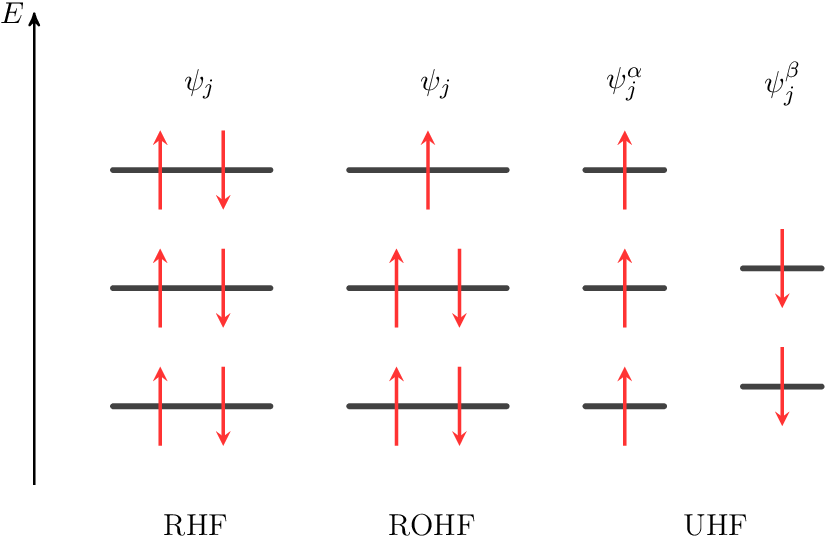
\includegraphics[width=0.5\linewidth]{Graphics/HF_Orb}
\caption{\textbf{Orbitales moléculaires et approches Hartree-Fock.} Choix de la méthode Hartree-Fock (RHF, ROHF, UHF) en fonction du remplissage ou de l'occupation des orbitales moléculaires. RHF est adapté aux systèmes à couches fermées, ROHF aux couches ouvertes, et UHF aux systèmes fortement magnétiques, mais au prix d'une complexité accrue et d'un risque de spin contamination.}
\label{fig:hforb}
\end{figure}

\begin{itemize}
    \item \textbf{Hartree-Fock restreint (RHF - Restricted HF)}.
    \begin{itemize}
        \item Utilisé pour les systèmes où \textbf{toutes les orbitales occupées sont doublées} (couches fermées), c’est-à-dire que chaque orbitale moléculaire contient une paire d’électrons de spins opposés.
        
        \item Les mêmes fonctions spatiales sont attribuées aux électrons de spin $\alpha$ et $\beta$.
        
        \item Convient aux molécules dans un \textbf{multiplicité de spin singulet} ($S = 0$), comme les molécules diamagnétiques.
    \end{itemize}
    
    \item \textbf{Hartree-Fock restreint pour les couches ouvertes (ROHF - Restricted Open-Shell HF)}.
    \begin{itemize}
        \item Adapté aux molécules à \textbf{couches ouvertes}, où certains électrons ne sont pas appariés.
        
        \item Les orbitales occupées par deux électrons restent symétriques comme en RHF), tandis que les orbitales contenant un seul électron sont traitées de manière spécifique.
        
        \item Permet de modéliser des systèmes avec une \textbf{multiplicité de spin non nulle} ($S > 0$),  comme les radicaux ou les atomes ayant un moment magnétique net.
    \end{itemize}

    \item \textbf{Hartree-Fock non restreint (UHF - Unrestricted HF)}.
    \begin{itemize}
        \item Utilisé pour les systèmes à \textbf{couches ouvertes}, notamment lorsque le spin total du système ne permet pas une solution symétrique.
        
        \item Contrairement à RHF et ROHF, les électrons de spin $\alpha$ et $\beta$ sont décrits par des \textbf{fonctions spatiales différentes}.
        
        \item Permet une plus grande flexibilité mais peut introduire un phénomène d’\textbf{instabilité de spin} (le spin-contamination), où la solution obtenue ne correspond pas exactement à l’état de spin souhaité.
    \end{itemize}
\end{itemize}

\subsubsection{Comparaison et choix du modèle Hartree-Fock}

Le choix entre RHF, ROHF et UHF dépend du type de molécule étudiée :
\begin{itemize}
    \item \textbf{RHF} est adapté aux molécules \textbf{fermées} sans électron non apparié (ex. \ch{H2}, \ch{CH4}).

    \item \textbf{ROHF} est souvent utilisé pour les systèmes avec \textbf{un nombre impair d’électrons} ou des \textbf{ions radicalaires} (ex. \ch{NO}, \ch{O2}).

    \item \textbf{UHF} est nécessaire pour les systèmes fortement magnétiques, où les électrons occupent des orbitales spatiales distinctes (ex. \textbf{métaux de transition, complexes paramagnétiques}).
\end{itemize}

Le tableau suivant résume les différences entre ces trois méthodes :

\begin{table}[h!]
    \centering
    \begin{tabular}{|p{2.cm}|p{5cm}|p{5cm}|p{3.cm}|}
        \hline
        \textbf{Méthode HF} & \textbf{Systèmes adaptés} & \textbf{Description des orbitales} & \textbf{Multiplicité de spin} \\
        \hline
        RHF  & Couches fermées & Identiques pour $\alpha$ et $\beta$ & $S=0$ \\
        \hline
        ROHF & Couches ouvertes (électrons non appariés) & Identiques sauf pour les non-appariés & $S>0$ \\
        \hline
        UHF  & Systèmes magnétiques ou couches ouvertes & Différentes pour $\alpha$ et $\beta$ & $S>0$ \\
        \hline
    \end{tabular}
    \caption{\textbf{Synthèse du choix de la méthode Hartree-Fock.} Comparaison des trois variantes de la méthode Hartree-Fock, en fonction de la structure électronique du système (couches fermées vs. couches ouvertes, magnétisme) et du type d'orbitales utilisées. Le choix de la méthode impacte la précision et le coût du calcul.}
\end{table}

En pratique, UHF est souvent préféré pour des \textbf{états excités ou fortement corrélés}, tandis que RHF et ROHF sont plus appropriés pour les calculs standards d'énergie fondamentale.

\subsection{Quelques limites des méthodes HF}

La méthode de Hartree-Fock présente certaines limites :
\begin{enumerate}
\item \textbf{Approximation du champ moyen}. La corrélation électronique est uniquement prise en compte par l’interaction d’échange.
\item \textbf{Absence de corrélation électronique dynamique}. Les interactions instantanées entre électrons ne sont pas modélisées.
    \item \textbf{Difficultés pour les systèmes fortement corrélés}. La méthide de HF est inefficace pour les molécules avec liaisons multiples ou états multi-déterminants.
\item \textbf{Sensibilité aux bases de fonction}. La précision des résultats de la méthode de HF dépend fortement du choix des bases de fonction utilisées pour décrire les orbitales électroniques.
\end{enumerate}

\section{\label{sec:Base} Choix de l'ensemble de bases}

L'équation de Schrödinger à plusieurs électrons est généralement résolue sur une base d'orbitales moléculaires exprimées sous la forme d'une \textbf{combinaison linéaire de ses orbitales atomiques (LCAO, Linear combination of atomic orbitals)}, 
\begin{equation}
     \phi_a(\mathbf{r}) =
     \sum_A^\mathrm{atomes}
     \sum_\alpha C^A_{\alpha a}
     \chi^A_{\alpha}(\mathbf{r} - \mathbf{R}_A) .
\end{equation}
où $\chi^A_{\alpha}(\mathbf{r} - \mathbf{R}_A)$ sont les \textbf{fonctions de base} centrées sur l’atome $A$, et $C^A_{\alpha a}$ sont les coefficients de la combinaison linéaire. Ces coefficients sont optimisés via le \textbf{principe variationnel}.

\subsection{Ensembles de bases traditionnels}

Les deux classes principales d'orbitales de base approximatives utilisées en chimie quantique sont :
\begin{itemize}
\item les \textbf{Slater-type orbitals (STOs)} basées sur le déterminant de Slater, construitent avec des fonctions exponentielles décroissantes
    \begin{equation}
        \chi_{\mathrm{STO}}(r) = e^{-\alpha r},
    \end{equation}
\item et les \textbf{orbitales cartésiennes de type Gaussien (GTO)}, construitent avec des fonctions Gaussiennes
    \begin{equation}
        \chi_{\mathrm{GTO}}(r) = e^{-\alpha r^2}.
    \end{equation}
  Ces orbitales facilitent le calcul des intégrales de recouvrement et sont donc plus couramment utilisées que les STO en chimie quantique computationnelle.
\end{itemize}

Les STO sont plus proches de la forme exacte des orbitales atomiques, mais les GTO permettent de simplifier les calculs d’intégrales électroniques. Un compromis entre ces deux approches consiste à combiner plusieurs GTO pour approximer une STO, donnant naissance aux bases \textbf{STO-nG} (Slater-Type Orbital – n Gaussians), où $n$ est le nombre de Gaussiennes utilisées dans l’approximation.

\subsection{Notations des ensembles de bases}

Les ensembles de bases sont constitués de plusieurs \textbf{primitives gaussiennes}. L'une des notations les plus explicites est celle de Pople :
\begin{itemize}
    \item Le \textbf{trait d'union (-)} sépare la référence aux orbitales centrales et de valence ;
    \item Les \textbf{chiffres} indiquent le nombre de primitives Gaussiennes utilisées ;
    \item La \textbf{lettre G} signifie que des Gaussiennes sont utilisées.
\end{itemize}

Par exemple, la base \texttt{6-31G} signifie :
\begin{itemize}
    \item 6 primitives Gaussiennes pour les orbitales internes.
    \item 3 primitives Gaussiennes pour les orbitales de valence.
    \item 1 primitive supplémentaire pour améliorer la flexibilité.
\end{itemize}
Cette notation s’étend aux bases plus complexes, comme \texttt{6-31G(d,p)}, où \textbf{(d,p)} indique l’ajout de fonctions de polarisation sur certains atomes.

En parallèle, d'autres familles d’ensembles de bases ont été développées pour répondre à des besoins spécifiques, notamment en méthodes post-Hartree-Fock.

\subsection{Bases correlation-consistent}

Les méthodes de chimie quantique avancées nécessitent des bases capables de capturer les effets de \textbf{corrélation électronique}. La famille \texttt{cc-pVXZ} (\textit{correlation-consistent polarized valence X-zeta}) est spécifiquement conçue pour cela :
\begin{itemize}
    \item \texttt{cc-pVDZ} : Double-$\zeta$, bonne précision pour les calculs préliminaires.
    \item \texttt{cc-pVTZ} : Triple-$\zeta$, plus précis pour les corrélations électroniques.
    \item \texttt{cc-pVQZ} : Quadruple-$\zeta$, nécessaire pour des énergies précises.
    \item \texttt{aug-cc-pVDZ} : Ajout de fonctions diffuses pour mieux représenter les anions et les états excités.
\end{itemize}

Plus d'informations, d'exemples et de discussions sur les GTO peuvent être trouvées dans ce  
\href{https://chem.libretexts.org/Courses/Pacific_Union_College/Quantum_Chemistry/11\%3A_Computational_Quantum_Chemistry/11.02\%3A_Gaussian_Basis_Sets}{lien}.

\subsection{Catégories d'ensembles de bases}

Les ensembles de bases modernes se répartissent en plusieurs catégories,
chacune adaptée à des besoins spécifiques en termes de précision et de coût
computationnel. Le tableau \ref{tab:basis_sets} résume les principales familles.

\begin{table}[h!]
    \centering
    \begin{tabular}{|l|p{8cm}|p{3cm}|}
        \hline
        \textbf{Catégorie} & \textbf{Description} & \textbf{Exemple} \\
        \hline
        Minimale & Une seule fonction de base par orbitale atomique occupée. & STO-3G \\
        \hline
        Double-$\zeta$ & Deux fonctions de base par orbitale atomique de valence. & 6-31G \\
        \hline
        Triple-$\zeta$ & Trois fonctions de base par orbitale atomique de valence. & 6-311G \\
        \hline
        Polarisation & Ajout de fonctions d'ordre supérieur pour mieux représenter la flexibilité des orbitales. & cc-pVDZ \\
        \hline
        Diffusion & Utilisation de fonctions étendues pour modéliser des électrons faiblement liés ou des états excités. & 6-31+G, aug-cc-pVDZ \\
        \hline
    \end{tabular}
    \caption{\textbf{Compromis précision-coût dans le choix des ensembles de bases.} Différentes catégories d'ensembles de bases, qui définissent comment les orbitales atomiques sont représentées mathématiquement. Le choix d'un ensemble de bases est un compromis entre la précision des résultats et les ressources de calcul nécessaires.}
    \label{tab:basis_sets}
\end{table}

\subsection{Bases de Karlsruhe}

Les ensembles \texttt{def2} de Karlsruhe offrent une alternative moderne aux bases de Pople et correlation-consistent. Elles couvrent l’ensemble du tableau périodique jusqu’au radon ($Z=86$) et intègrent des
\textbf{potentiels de noyau effectif (ECP)} pour les éléments lourds. Trois niveaux de précision sont disponibles :
\begin{itemize}
    \item \textbf{def2-SVP} : Base compacte, adaptée aux calculs rapides (équivalent à \texttt{6-31G**}).
    \item \textbf{def2-TZVP} : Triple-$\zeta$ avec polarisation, bon compromis précision/coût.
    \item \textbf{def2-QZVP} : Quadruple-$\zeta$, utilisé pour des études très précises.
\end{itemize}
L'utilisation de bases \texttt{def2} est souvent privilégiée en \textbf{DFT (Density Functional Theory)} et en \textbf{calculs post-Hartree-Fock}.

\subsection{Critères pour choisir un ensemble de bases}

Le choix optimal dépend du système étudié et des exigences du calcul. En règle générale pour,
\begin{itemize}
    \item \textbf{Études rapides :} \texttt{6-31G}, \texttt{def2-SVP}.
    \item \textbf{Chimie de la valence :} \texttt{cc-pVDZ}, \texttt{def2-TZVP}.
    \item \textbf{Calculs précis :} \texttt{cc-pVTZ}, \texttt{def2-QZVP}.
    \item \textbf{Anions et états excités :} \texttt{aug-cc-pVDZ}, \texttt{def2-TZVPPD}.
    \item \textbf{Effets relativistes :} bases avec \textbf{potentiels de noyau effectif (ECP)}, ex. \texttt{LANL2DZ}.
\end{itemize}

En augmentant la taille de l’ensemble de bases, l’approximation obtenue  se rapproche de la fonction d’état exacte :
\begin{equation}
\langle \Phi_{\text{approx}} | \mathtt{H} | \Phi_{\text{approx}} \rangle \geq  \epsilon_{\text{true}}.
\end{equation}
Cependant, une base plus grande implique une augmentation des coûts de calcul. Il est donc essentiel de trouver un équilibre optimal.

\subsection{Conclusion}

Le choix d’un ensemble de bases est un facteur déterminant en chimie quantique computationnelle. Un compromis doit être trouvé entre la précision souhaitée et les ressources disponibles. Les bases modernes, comme \texttt{def2} et \texttt{cc-pVXZ}, offrent des solutions flexibles adaptées à divers niveaux de calcul. En sélectionnant soigneusement une base appropriée, on optimise le rapport coût-précision pour les études moléculaires.

\section{Conclusion - Premiers pas dans la modélisation moléculaire}

Dans ce chapitre, nous avons exploré les fondements de la modélisation de la structure électronique des molécules, en nous concentrant sur l'approximation de Born-Oppenheimer et la méthode de Hartree-Fock. En résumé, voici les étapes clés de cette approche en \textit{première approximation} :
\begin{enumerate}
    \item \textbf{Approximation de Born-Oppenheimer.} On considère que les noyaux sont fixes et on se concentre sur le mouvement des électrons dans le potentiel créé par ces noyaux fixes.
    \item \textbf{Choix d'une base d'orbitales.} On sélectionne un ensemble de fonctions de base (par exemple, STO-3G, 6-31G*) pour représenter les orbitales atomiques.
    \item \textbf{Construction du déterminant de Slater.} On construit une fonction d'état multi-électronique antisymétrique en utilisant un déterminant de Slater.
    \item \textbf{Méthode de Hartree-Fock (SCF).} On utilise une procédure itérative pour optimiser les orbitales moléculaires en considérant que chaque électron se déplace dans un champ moyen créé par les autres.
\end{enumerate}

\textbf{Un choix déterminant : approximations et bases}

Il est essentiel de comprendre que cette procédure repose sur des approximations. La méthode Hartree-Fock néglige une partie importante de la corrélation électronique, ce qui peut affecter la précision des résultats. De plus, le choix de la base d'orbitales a un impact direct sur la qualité de la modélisation et sur le temps de calcul.

Le choix des approximations et de l'ensemble de bases dépend fortement des objectifs de l'étude :
\begin{itemize}
    \item Pour des \textbf{calculs rapides et qualitatifs}, on peut utiliser une base minimale (ex. STO-3G).
    \item Pour des \textbf{calculs plus précis}, on utilisera des bases étendues avec des fonctions de polarisation (ex. 6-31G*, cc-pVDZ).
    \item Si l'objectif est d'\textbf{étudier des propriétés spécifiques} (anions, états excités), on choisira une base adaptée (ex. aug-cc-pVDZ).
\end{itemize}
Comprendre ces compromis et les limitations de l'approche Hartree-Fock est essentiel pour interpréter correctement les résultats et pour choisir des méthodes plus avancées si nécessaire. Dans les chapitres suivants, nous explorerons ces méthodes post-Hartree-Fock qui visent à inclure la corrélation électronique et à améliorer la précision de la modélisation.

\end{document}
